%!TeX program = xelatex
\documentclass[12pt,hyperref,a4paper,UTF8]{ctexart}
\usepackage{HDUReport}
\usepackage{listings}
\usepackage{xcolor}
\usepackage{graphicx}
\usepackage{setspace}
\usepackage{float}
\setstretch{1.5} % 设置全局行距为1.5倍

\usepackage{enumitem} % 载入enumitem包以便自定义列表环境
\setlist[itemize]{itemsep=0pt, parsep=0pt} % 设置itemize环境的项目间距和段落间距

\setmainfont{Times New Roman} % 英文正文为Times New Roman

%封面页设置
{   
    %标题
    \title{ 
        \vspace{1cm}
        \heiti \Huge \textbf{电子信息虚拟仿真实验报告} \par
        \vspace{1cm} 
        \heiti \Large {\underline{忆阻器实验3:忆阻器脉冲响应}   } 
        \vspace{3cm}
    
    }

    \author{
        \vspace{0.5cm}
        \kaishu\Large 学院\ \dlmu[9cm]{卓越学院} \\ %学院
        \vspace{0.5cm}
        \kaishu\Large 学号\ \dlmu[9cm]{23040447} \\ %班级
        \vspace{0.5cm}
        \kaishu\Large 姓名\ \dlmu[9cm]{陈文轩} \qquad  \\ %学号
        \vspace{0.5cm}
        \kaishu\Large 专业\ \dlmu[9cm]{智能硬件与系统(电子信息工程)} \qquad \\ %姓名 
    }
        
    \date{\today} % 默认为今天的日期,可以注释掉不显示日期
}
%%------------------------document环境开始------------------------%%
\begin{document}

%%-----------------------封面--------------------%%
\cover
\thispagestyle{empty} % 首页不显示页码
%%------------------摘要-------------%%
%\newpage
%\begin{abstract}




%\end{abstract}

%\thispagestyle{empty} % 首页不显示页码

%%--------------------------目录页------------------------%%
% \newpage
% \tableofcontents
% \thispagestyle{empty} % 目录不显示页码

%%------------------------正文页从这里开始-------------------%
\newpage
\setcounter{page}{1} % 让页码从正文开始编号

%%可选择这里也放一个标题
%\begin{center}
%    \title{ \Huge \textbf{{标题}}}
%\end{center}

\section{实验记录}

\begin{table}[H]
    \centering
    \caption{幅度 -1V}
    \begin{tabular}{|c|c|c|c|}
        \hline
        脉宽(us) & 5 & 50 & 100 \\ \hline
        忆阻值($\Omega$) &2.339E-10 &2.299E-9 &4.652E-9 \\ \hline
        耗能(J) &11281 &11646 &11392 \\ \hline
    \end{tabular}
\end{table}

\begin{table}[H]
    \centering
    \caption{幅度 -0.5V}
    \begin{tabular}{|c|c|c|c|}
        \hline
        脉宽(us) & 5 & 50 & 100 \\ \hline
        忆阻值($\Omega$) &11614 &11189 &11281 \\ \hline
        耗能(J) &5.757E-11 &5.871E-10 &1.169E-9 \\ \hline
    \end{tabular}
\end{table}

\begin{table}[H]
    \centering
    \caption{幅度 0.5V}
    \begin{tabular}{|c|c|c|c|}
        \hline
        脉宽(us) & 5 & 50 & 100 \\ \hline
        忆阻值($\Omega$) & 10918& 11099& 10918 \\ \hline
        耗能(J) &1.189E-9 &5.897E-10& 1.189E-9 \\ \hline
    \end{tabular}
\end{table}

\begin{table}[H]
    \centering
    \caption{幅度 1V}
    \begin{tabular}{|c|c|c|c|}
        \hline
        脉宽(us) & 5 & 50 & 100 \\ \hline
        忆阻值($\Omega$) & 10873&11392 &10722 \\ \hline
        耗能(J) & 4.768E-12&2.326E-9&4.803E-9 \\ \hline
    \end{tabular}
\end{table}




\section{上传远程平台截图}


\begin{figure}[H]
    \centering
    \begin{minipage}{1\textwidth}
        \centering
        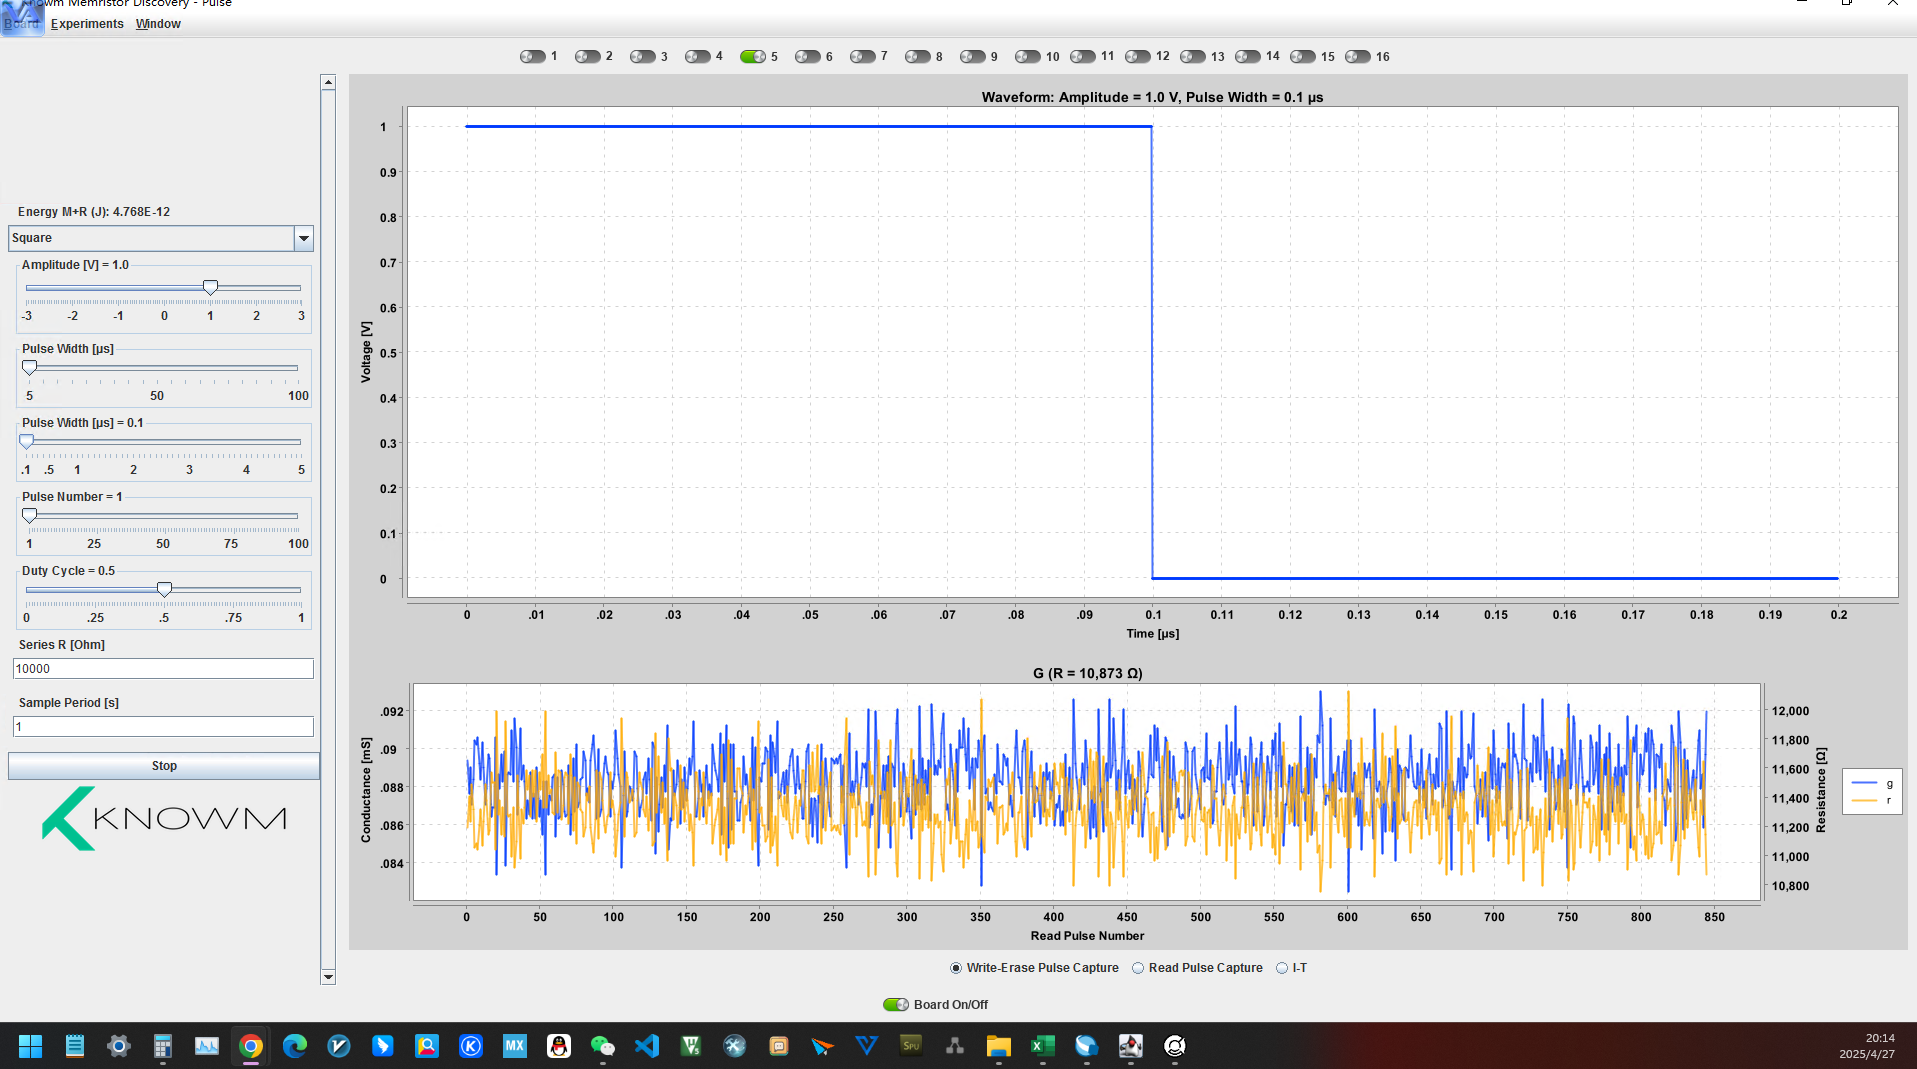
\includegraphics[width=1\textwidth]{figures/U1T5.png}
        \caption{U=1,T=5,实验记录}
        \label{fig:system_block_diagram}
    \end{minipage}
\end{figure}

\begin{figure}[H]
    \centering
    \begin{minipage}{1\textwidth}
        \centering
        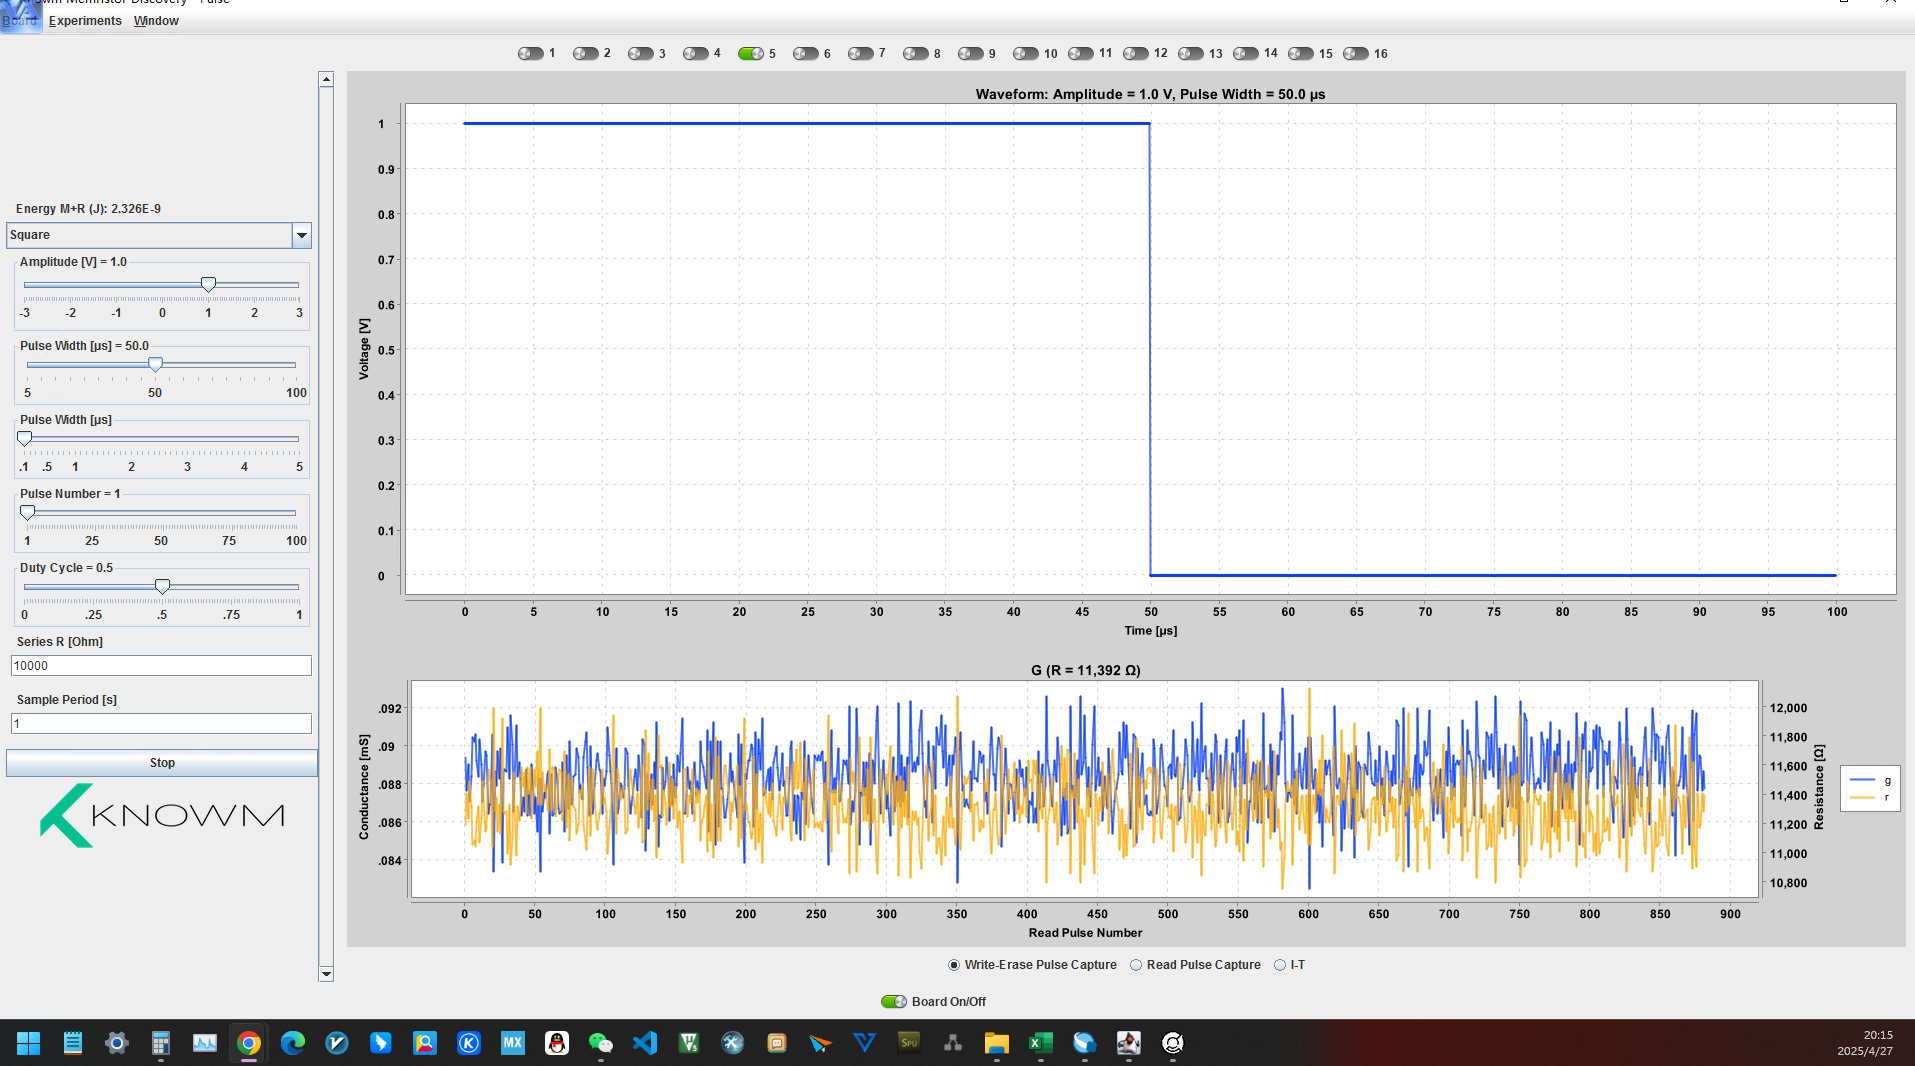
\includegraphics[width=1\textwidth]{figures/U1T50.png}
        \caption{U=1,T=50,实验记录}
        \label{fig:system_block_diagram}
    \end{minipage}
\end{figure}

\begin{figure}[H]
    \centering
    \begin{minipage}{1\textwidth}
        \centering
        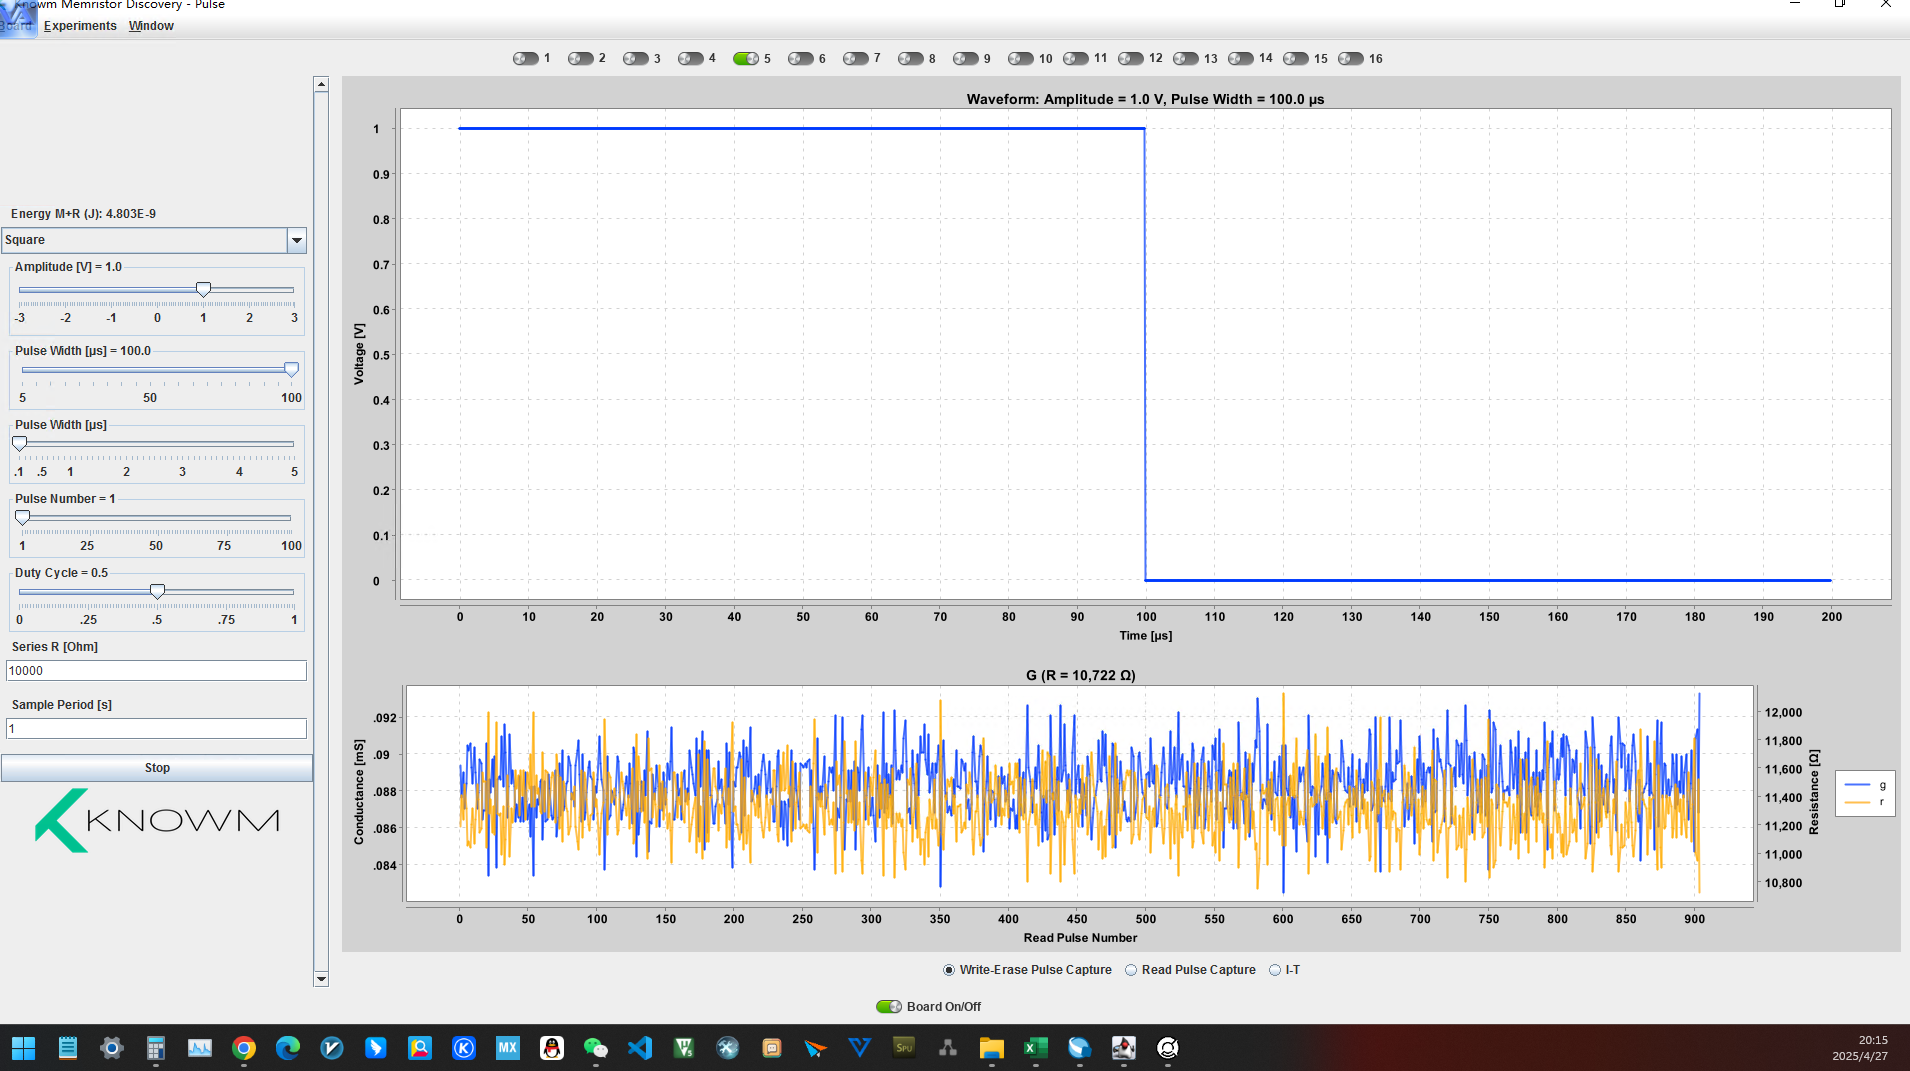
\includegraphics[width=1\textwidth]{figures/U1T100.png}
        \caption{U=1,T=100,实验记录}
        \label{fig:system_block_diagram}
    \end{minipage}
\end{figure}

\begin{figure}[H]
    \centering
    \begin{minipage}{1\textwidth}
        \centering
        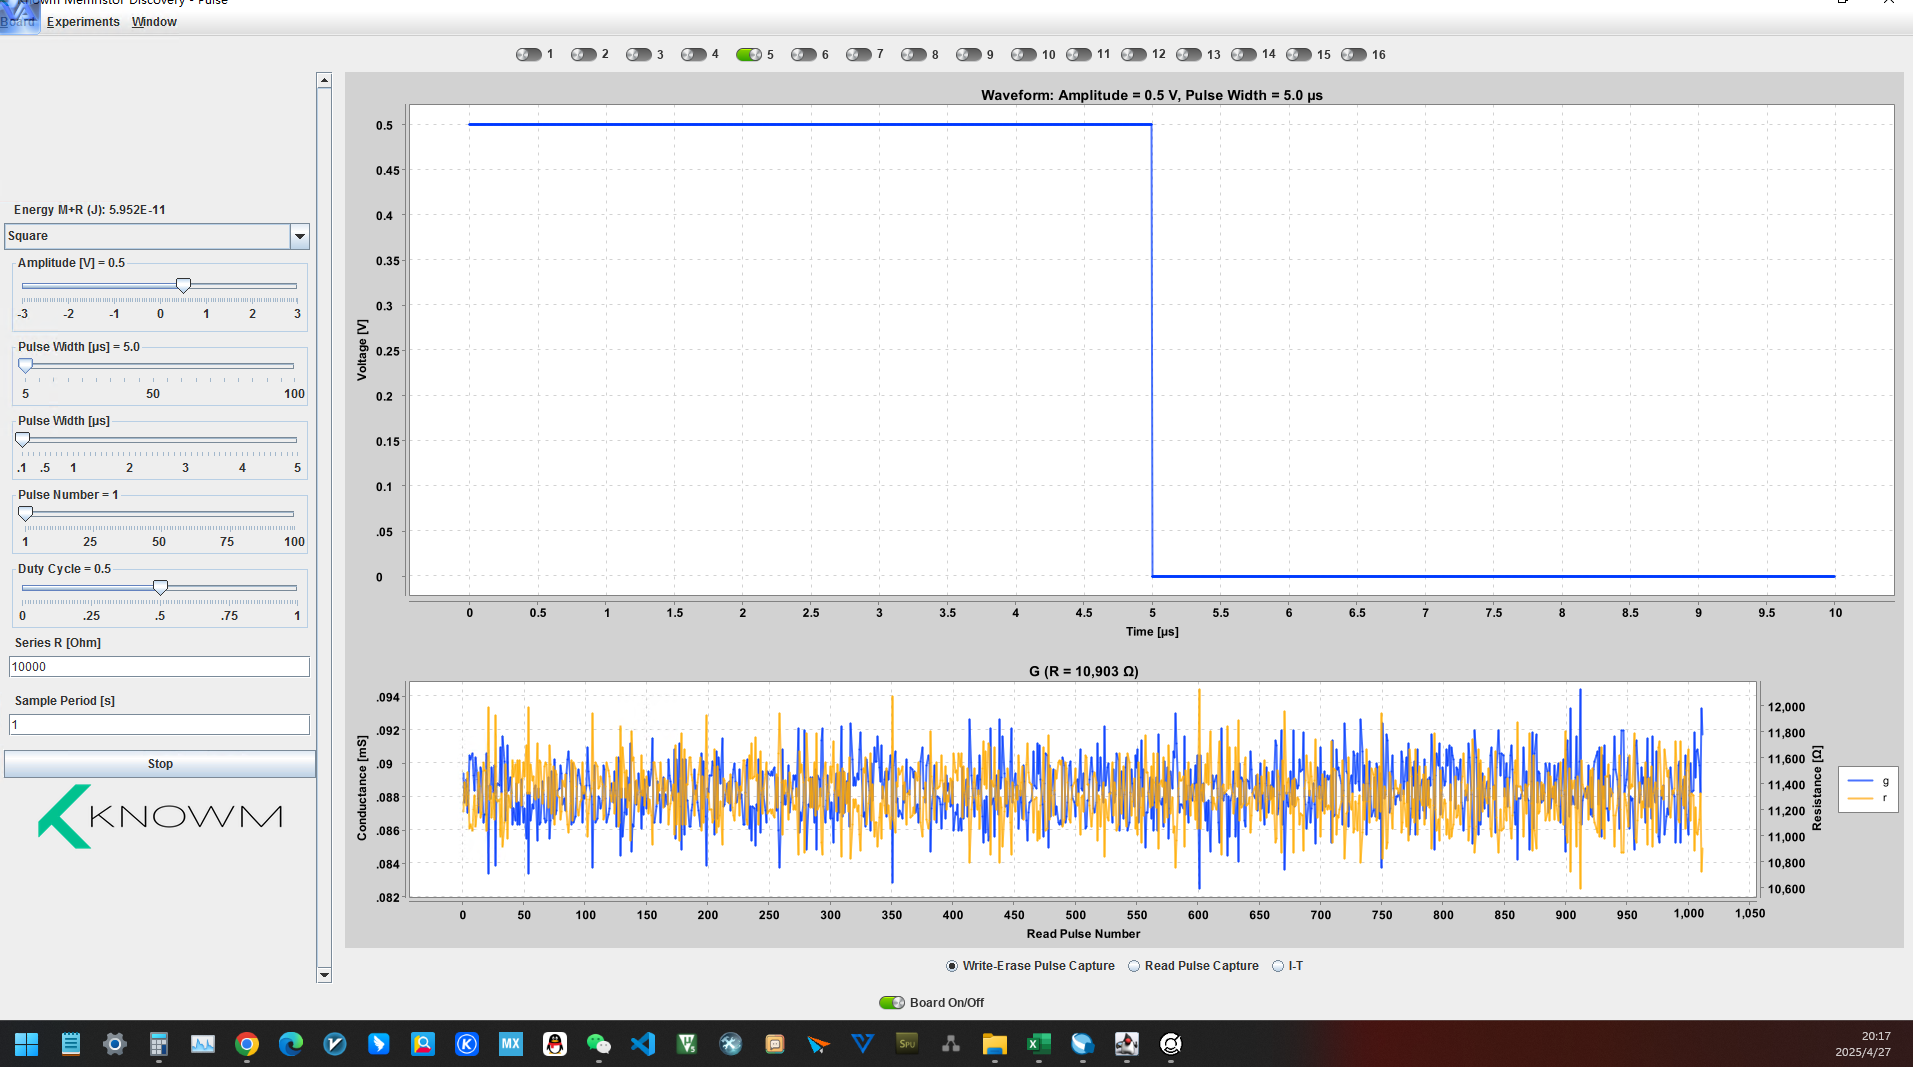
\includegraphics[width=1\textwidth]{figures/U05T5.png}
        \caption{U=0.5,T=5,实验记录}
        \label{fig:U05T5}
    \end{minipage}
\end{figure}

\begin{figure}[H]
    \centering
    \begin{minipage}{1\textwidth}
        \centering
        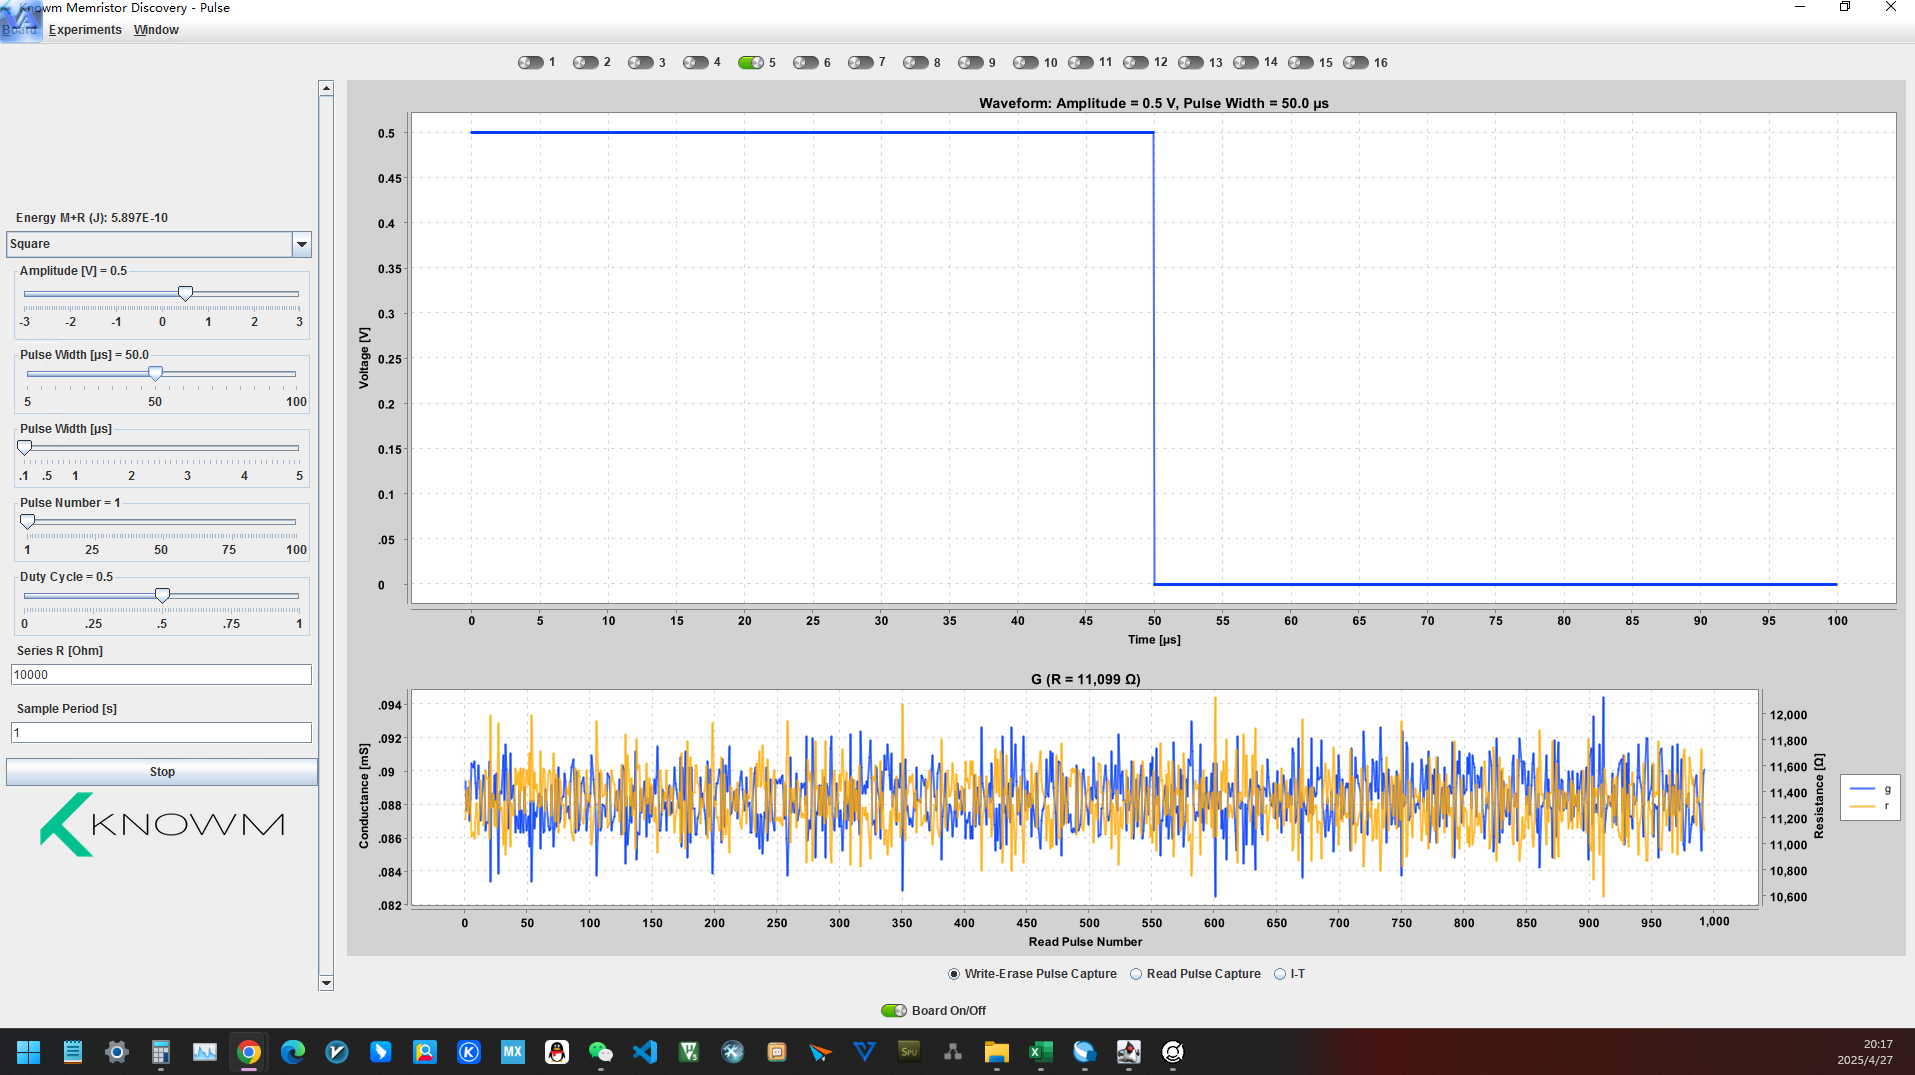
\includegraphics[width=1\textwidth]{figures/U05T50.png}
        \caption{U=0.5,T=50,实验记录}
        \label{fig:U05T50}
    \end{minipage}
\end{figure}

\begin{figure}[H]
    \centering
    \begin{minipage}{1\textwidth}
        \centering
        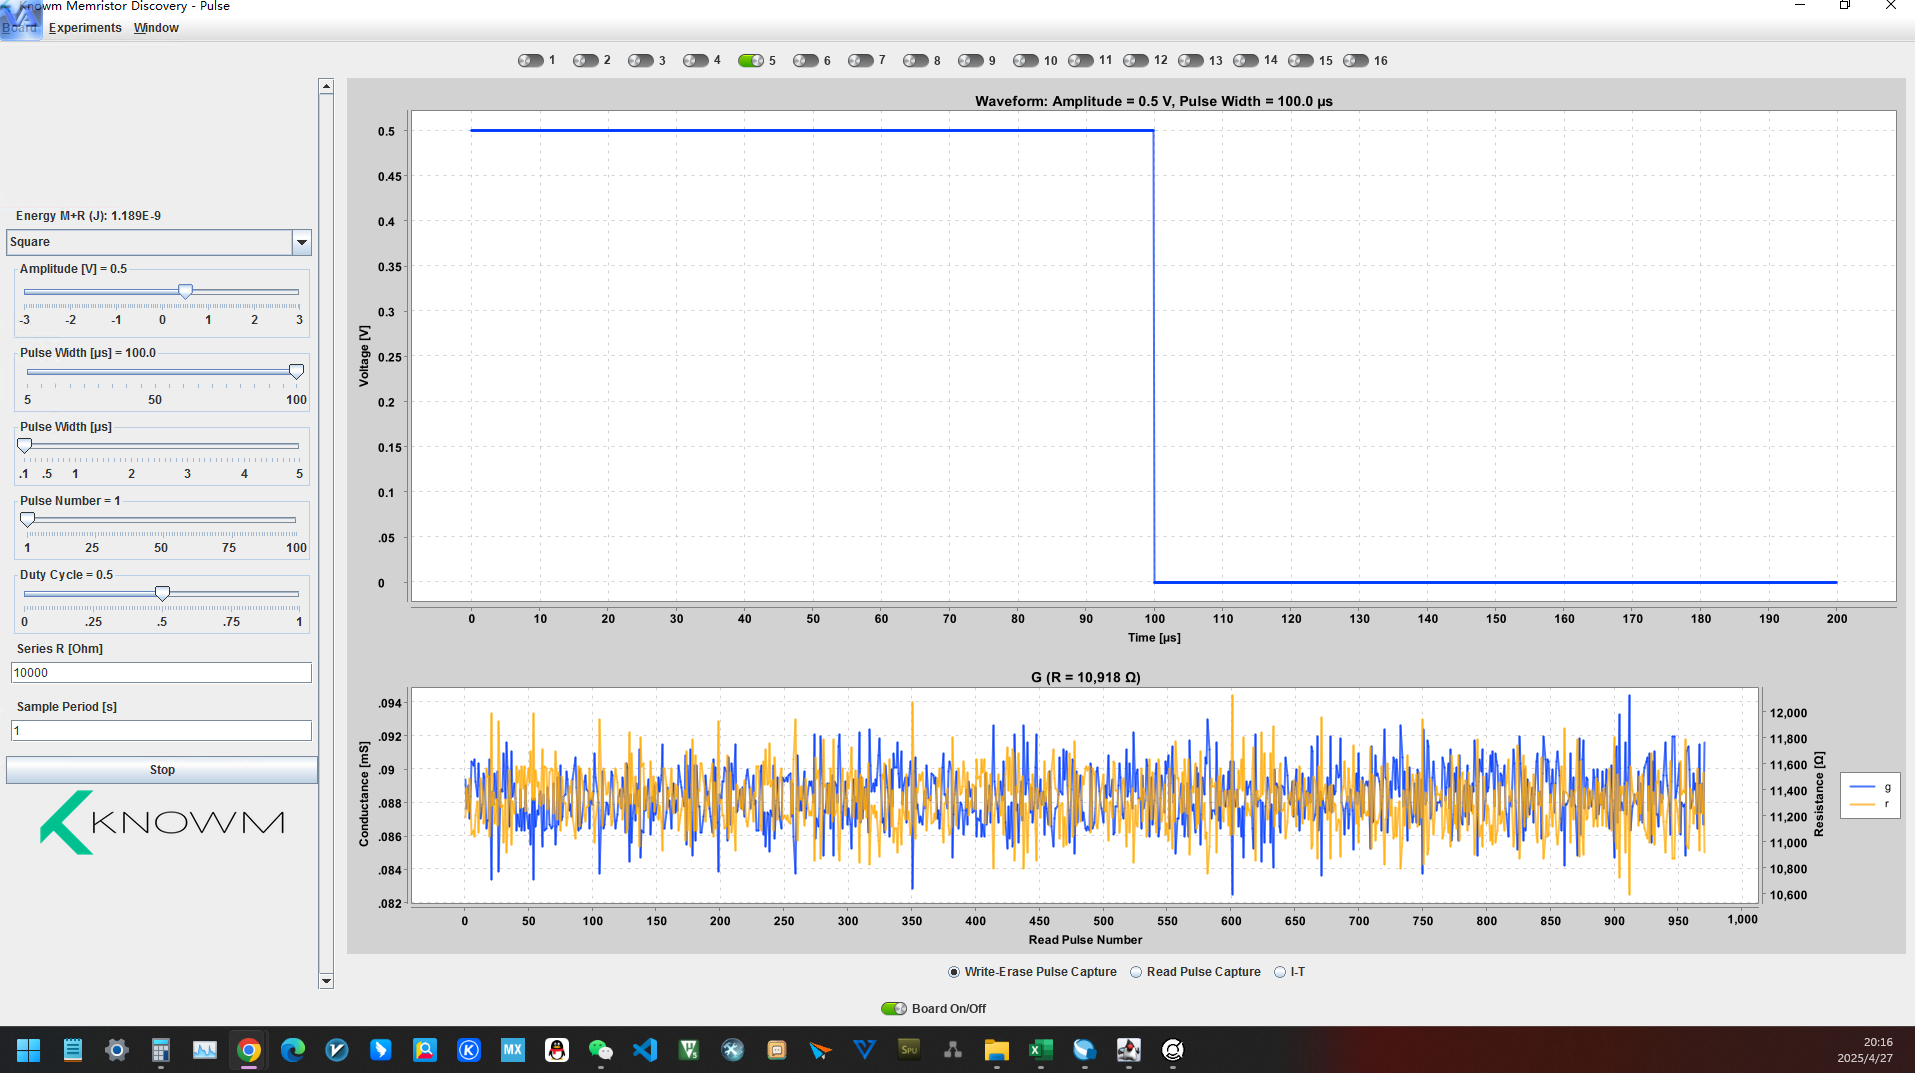
\includegraphics[width=1\textwidth]{figures/U05T100.png}
        \caption{U=0.5,T=100,实验记录}
        \label{fig:U05T100}
    \end{minipage}
\end{figure}

\begin{figure}[H]
    \centering
    \begin{minipage}{1\textwidth}
        \centering
        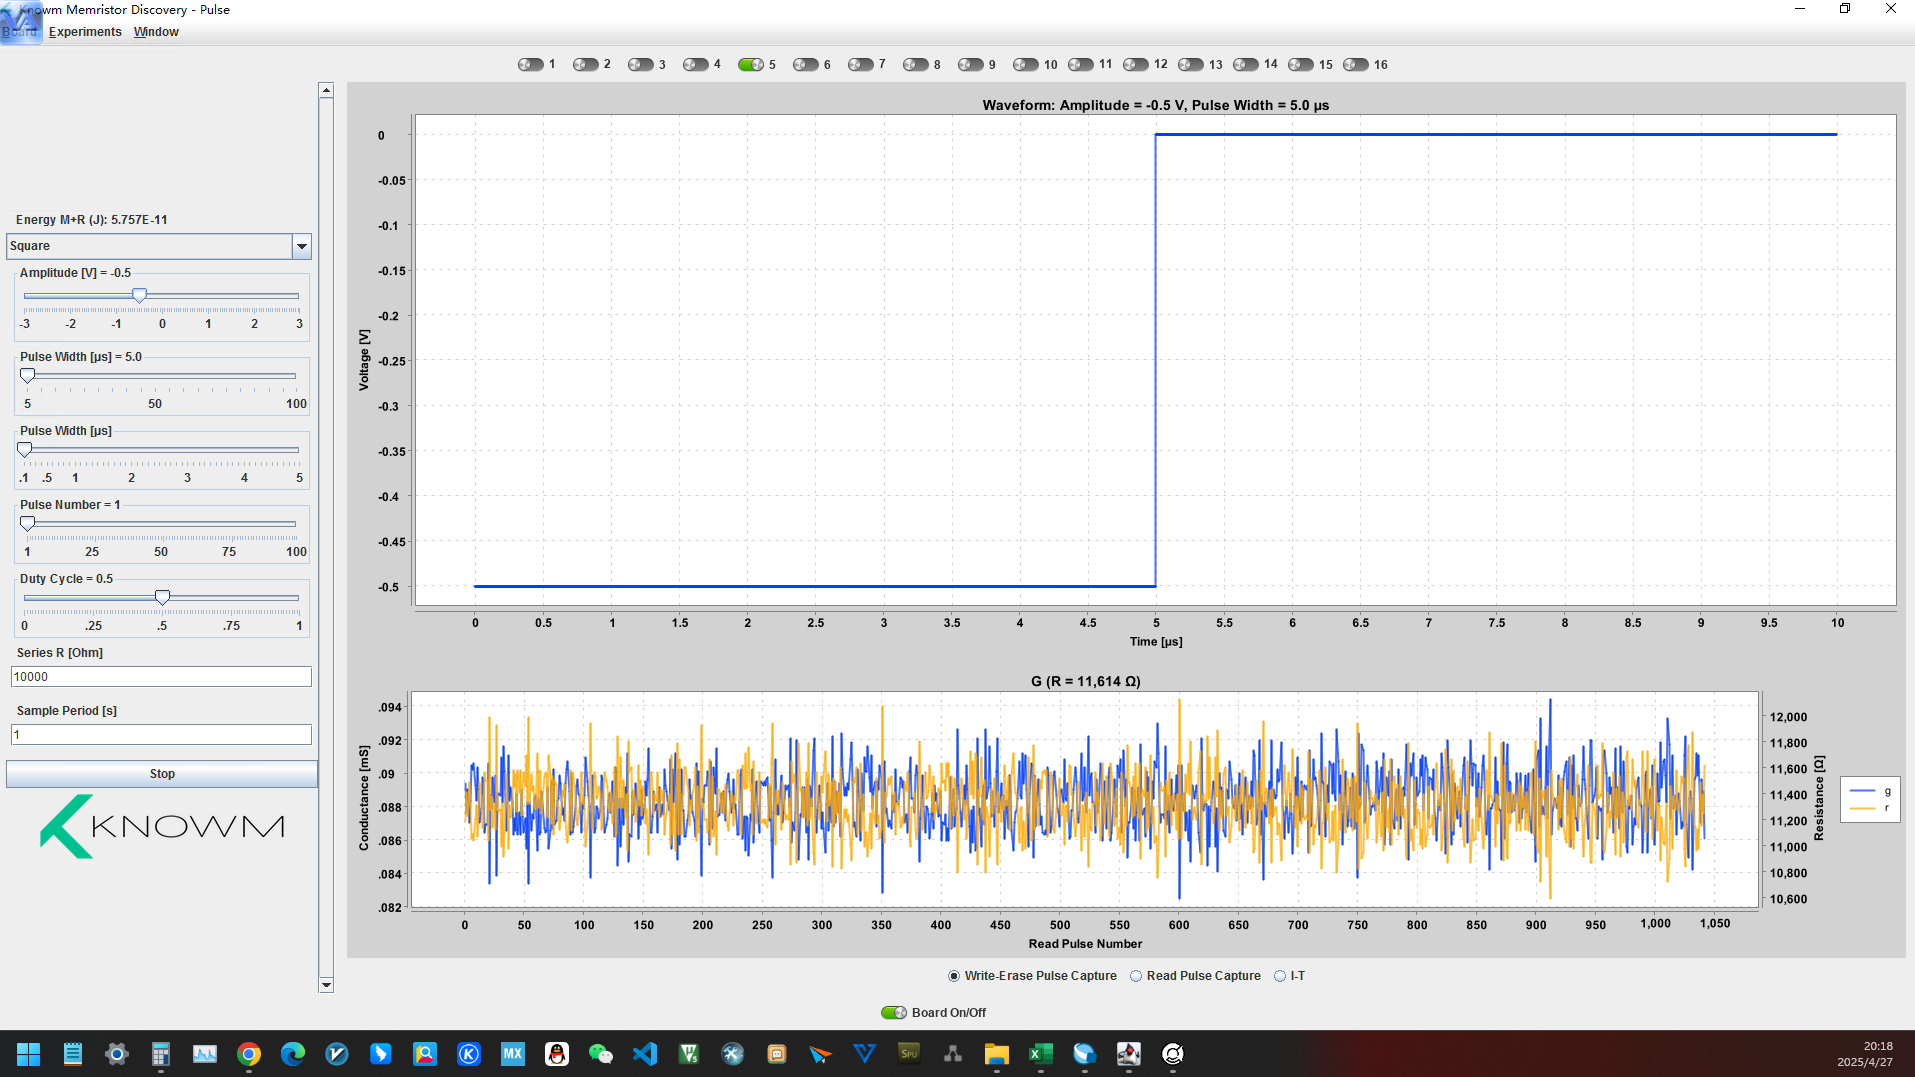
\includegraphics[width=1\textwidth]{figures/U-05T5.png}
        \caption{U=-0.5,T=5,实验记录}
        \label{fig:U-05T5}
    \end{minipage}
\end{figure}

\begin{figure}[H]
    \centering
    \begin{minipage}{1\textwidth}
        \centering
        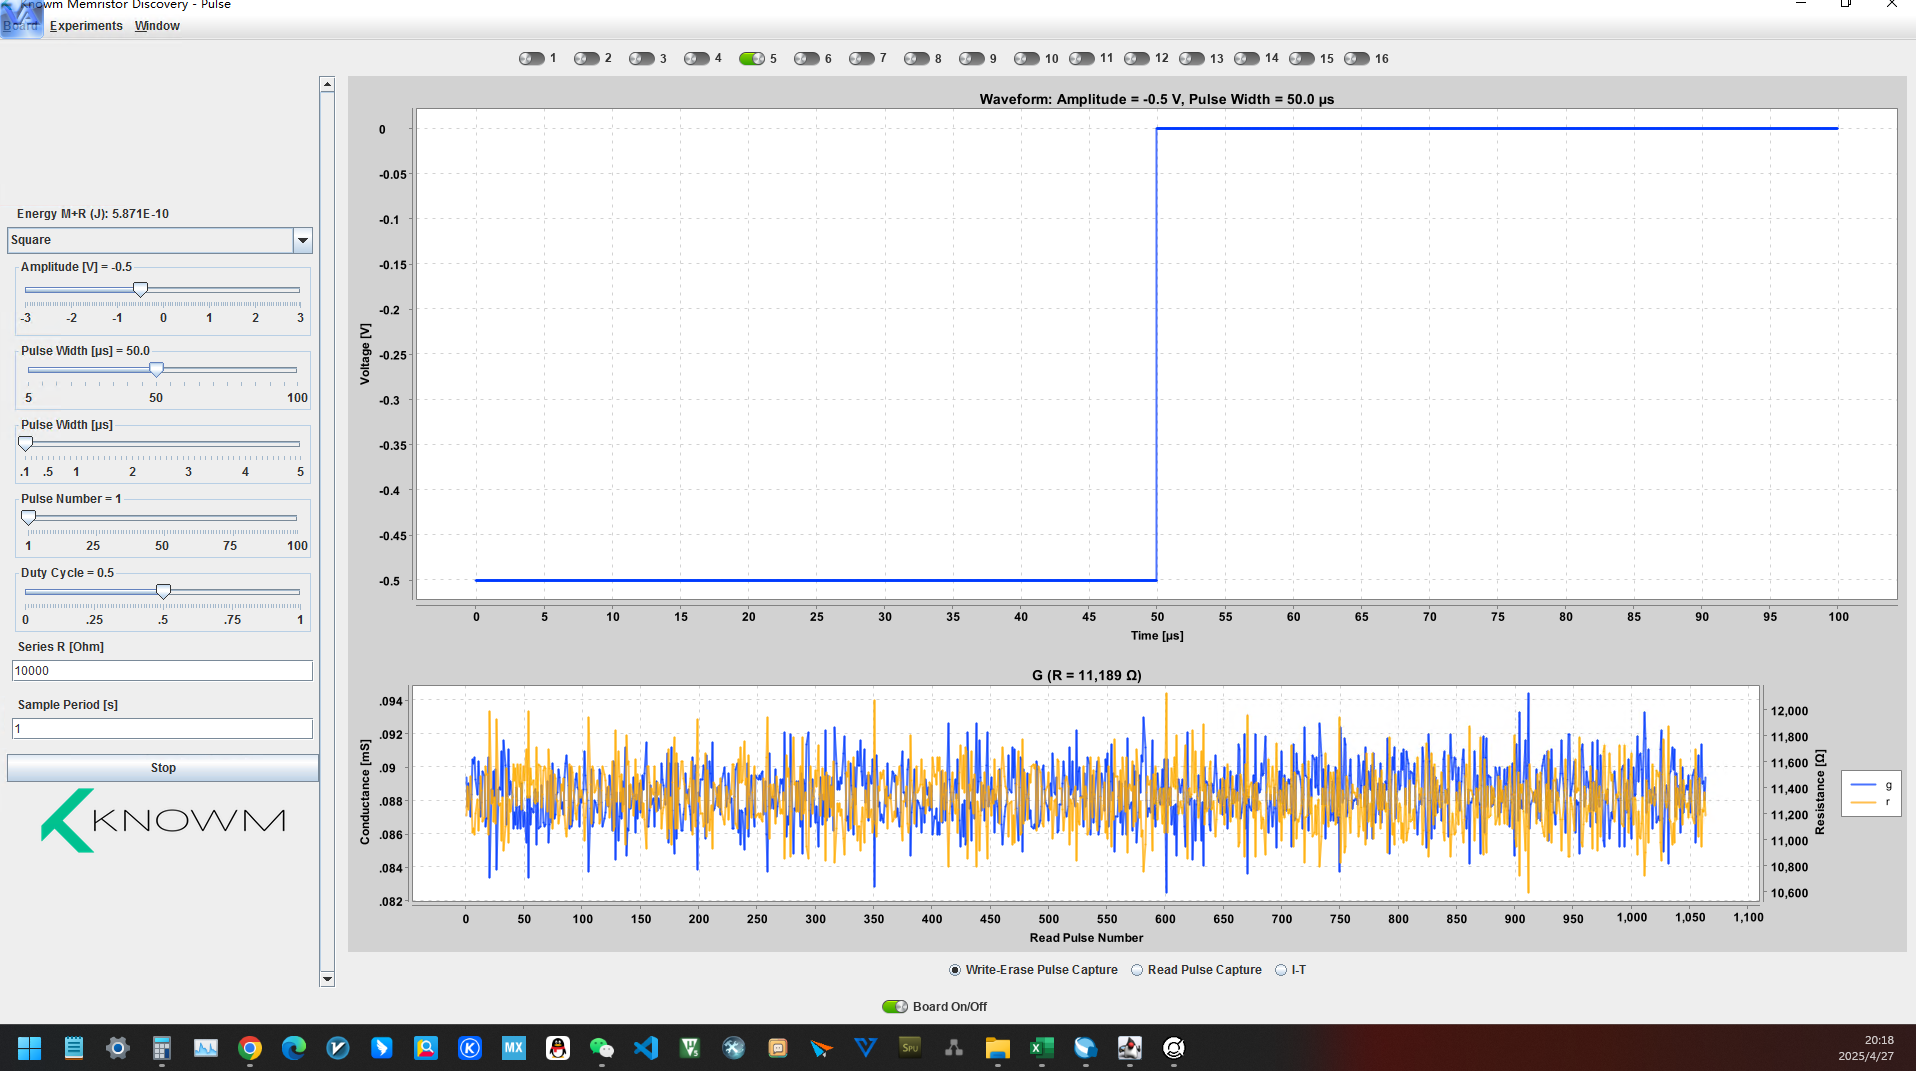
\includegraphics[width=1\textwidth]{figures/U-05T50.png}
        \caption{U=-0.5,T=50,实验记录}
        \label{fig:U-05T50}
    \end{minipage}
\end{figure}

\begin{figure}[H]
    \centering
    \begin{minipage}{1\textwidth}
        \centering
        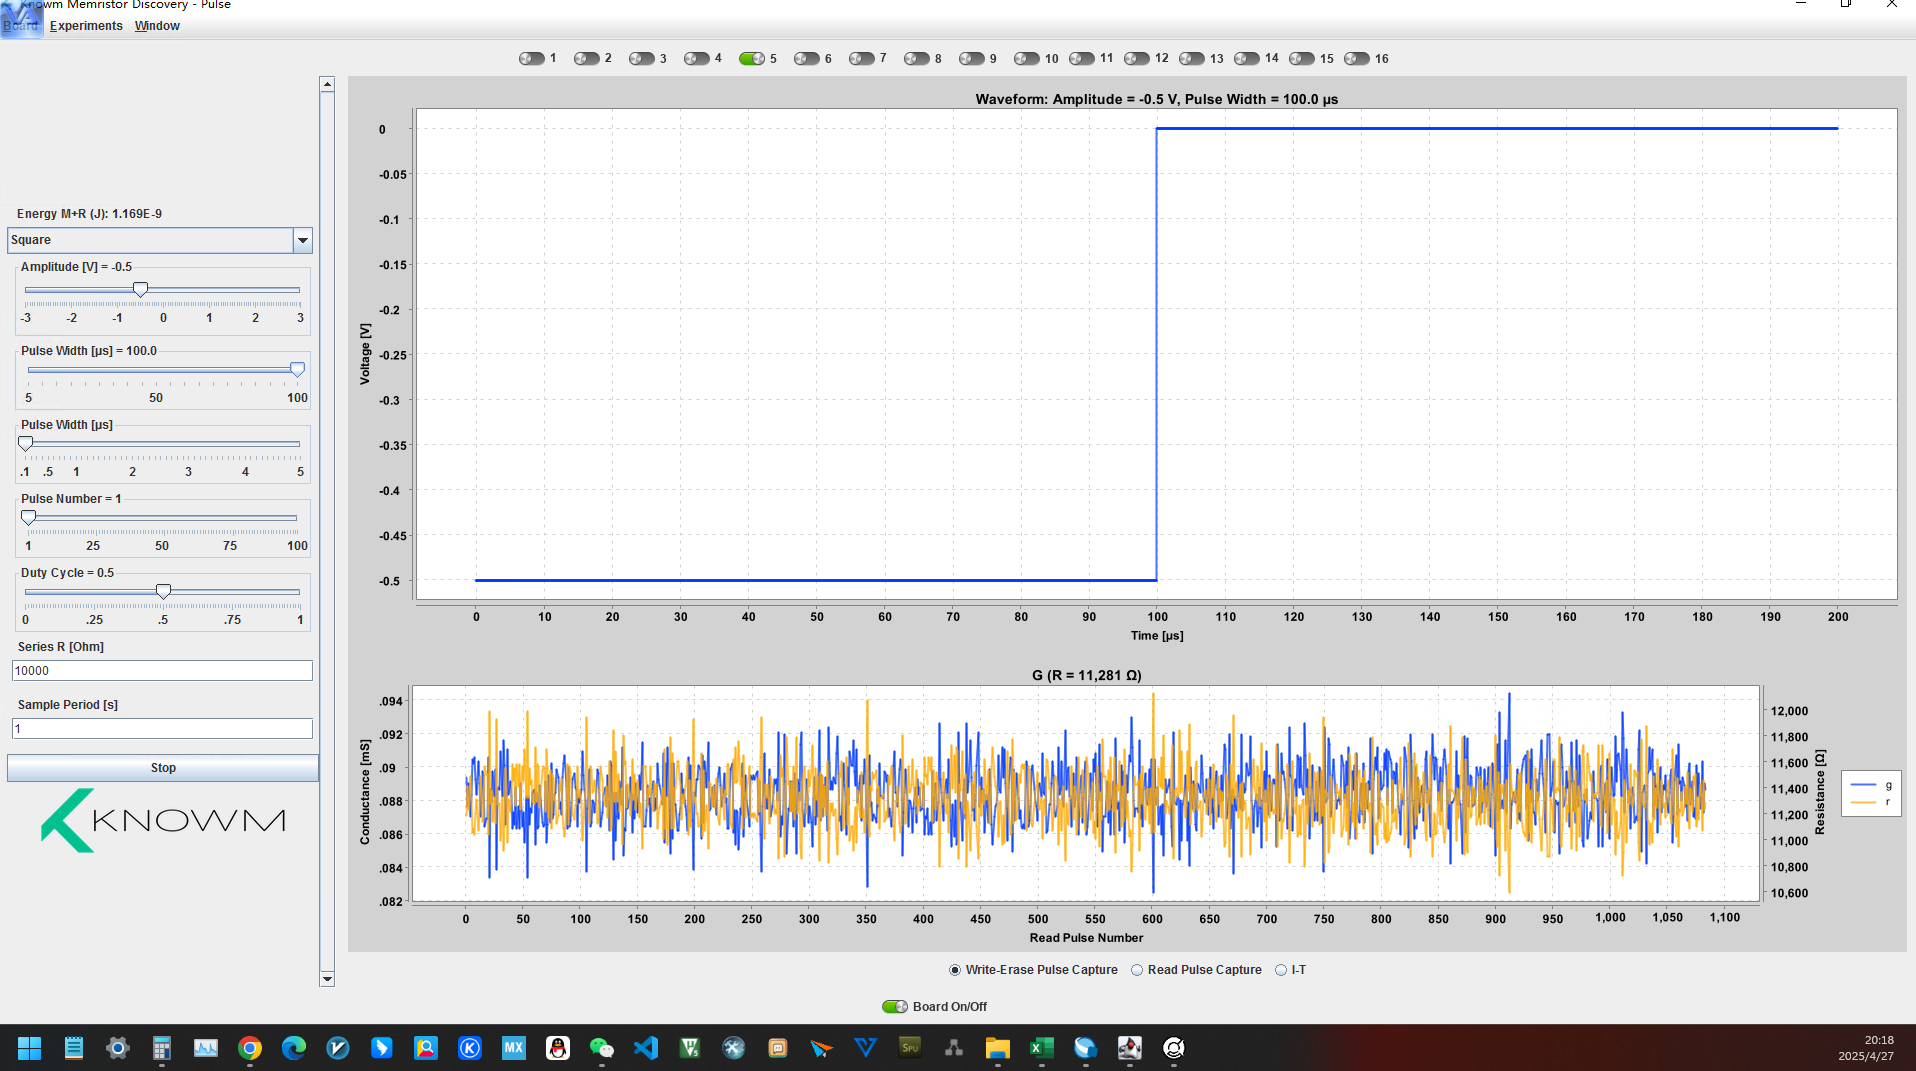
\includegraphics[width=1\textwidth]{figures/U-05T100.png}
        \caption{U=-0.5,T=100,实验记录}
        \label{fig:U-05T100}
    \end{minipage}
\end{figure}

\begin{figure}[H]
    \centering
    \begin{minipage}{1\textwidth}
        \centering
        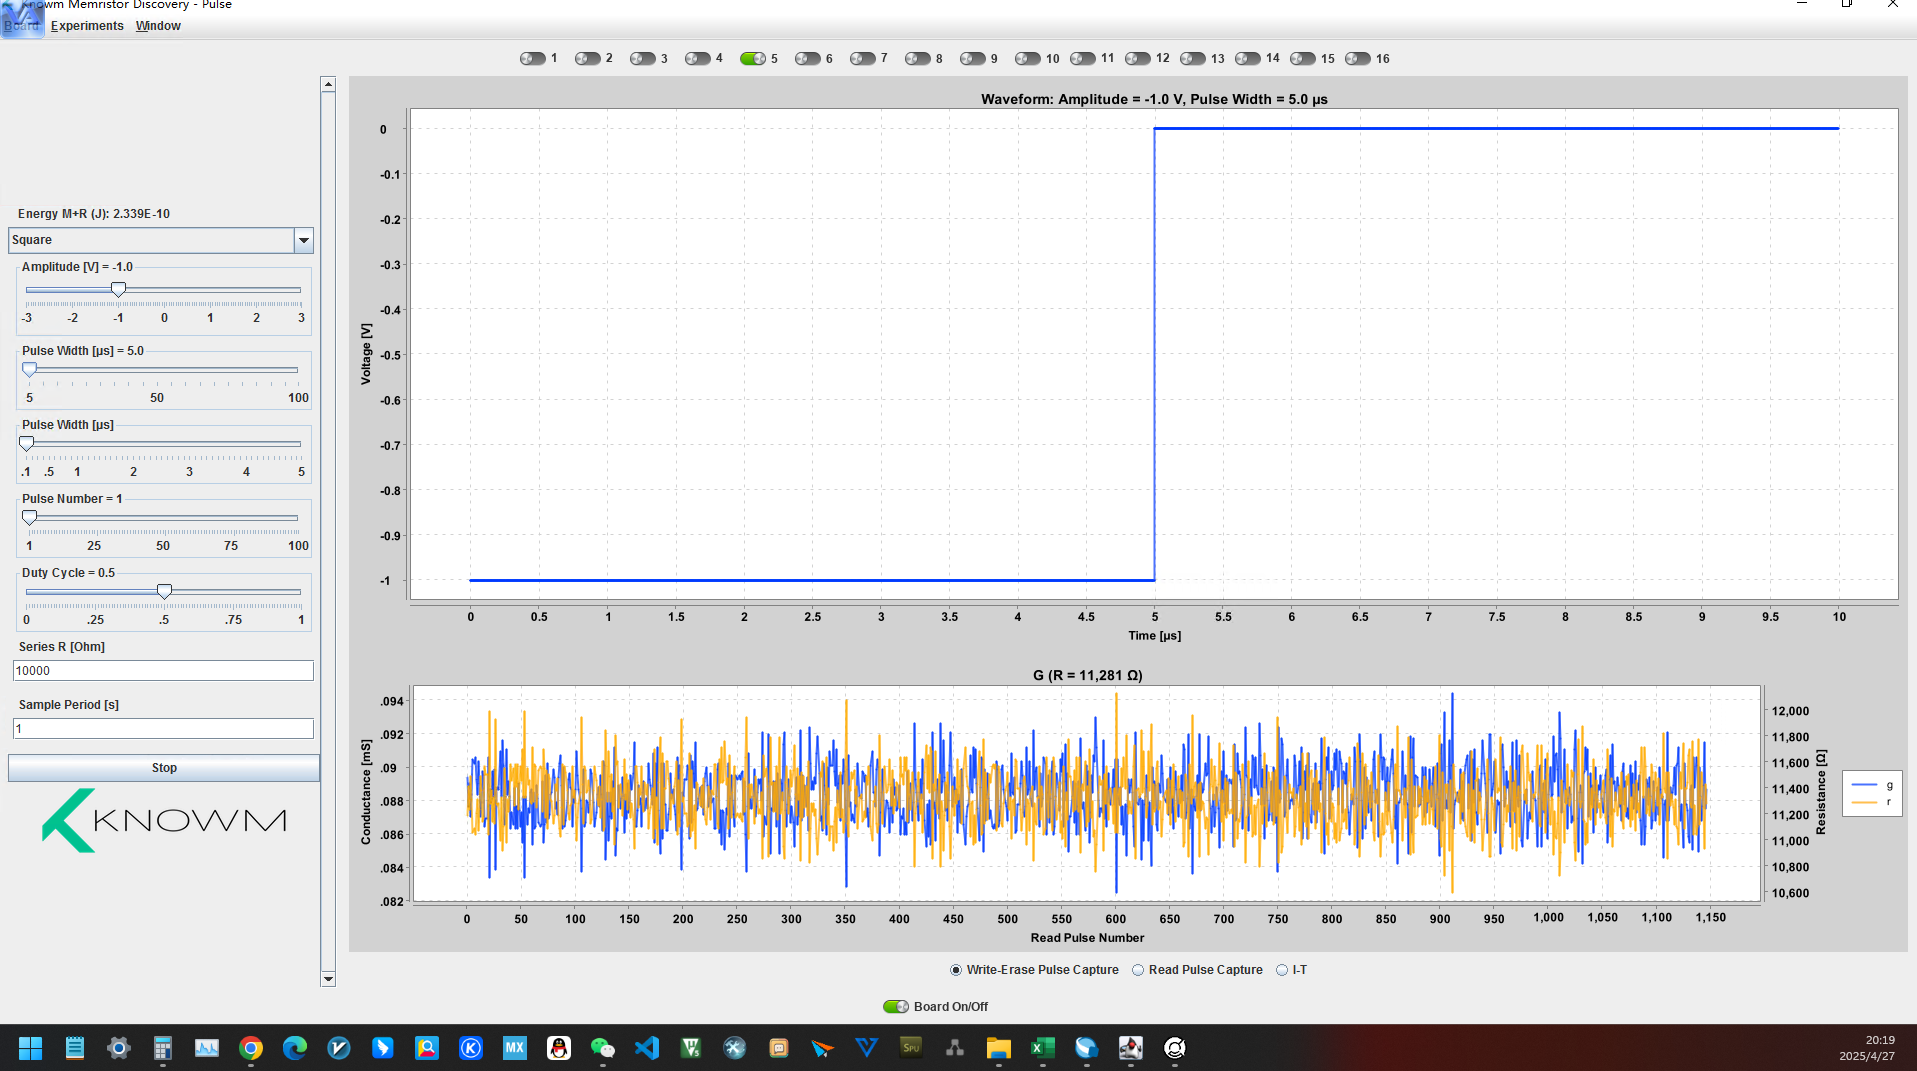
\includegraphics[width=1\textwidth]{figures/U-1T5.png}
        \caption{U=-1,T=5,实验记录}
        \label{fig:U-1T5}
    \end{minipage}
\end{figure}

\begin{figure}[H]
    \centering
    \begin{minipage}{1\textwidth}
        \centering
        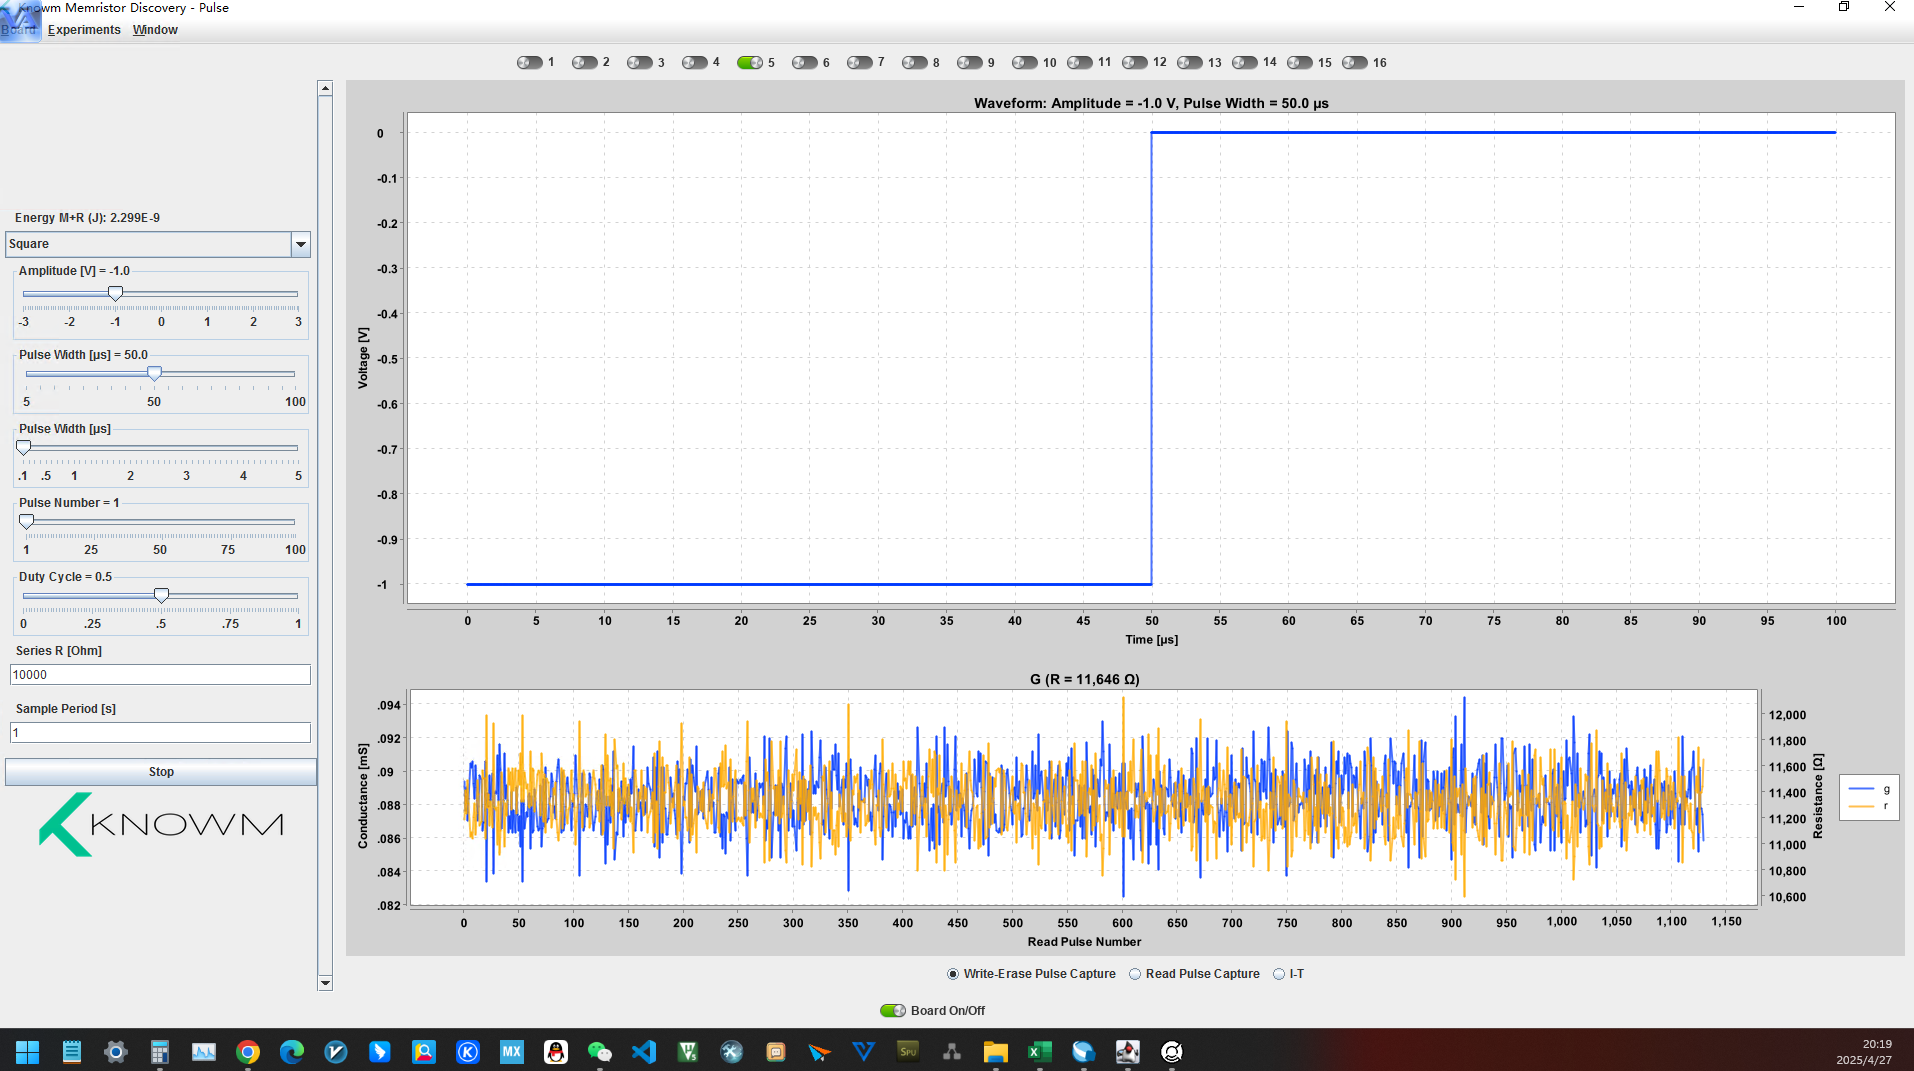
\includegraphics[width=1\textwidth]{figures/U-1T50.png}
        \caption{U=-1,T=50,实验记录}
        \label{fig:U-1T50}
    \end{minipage}
\end{figure}

\begin{figure}[H]
    \centering
    \begin{minipage}{1\textwidth}
        \centering
        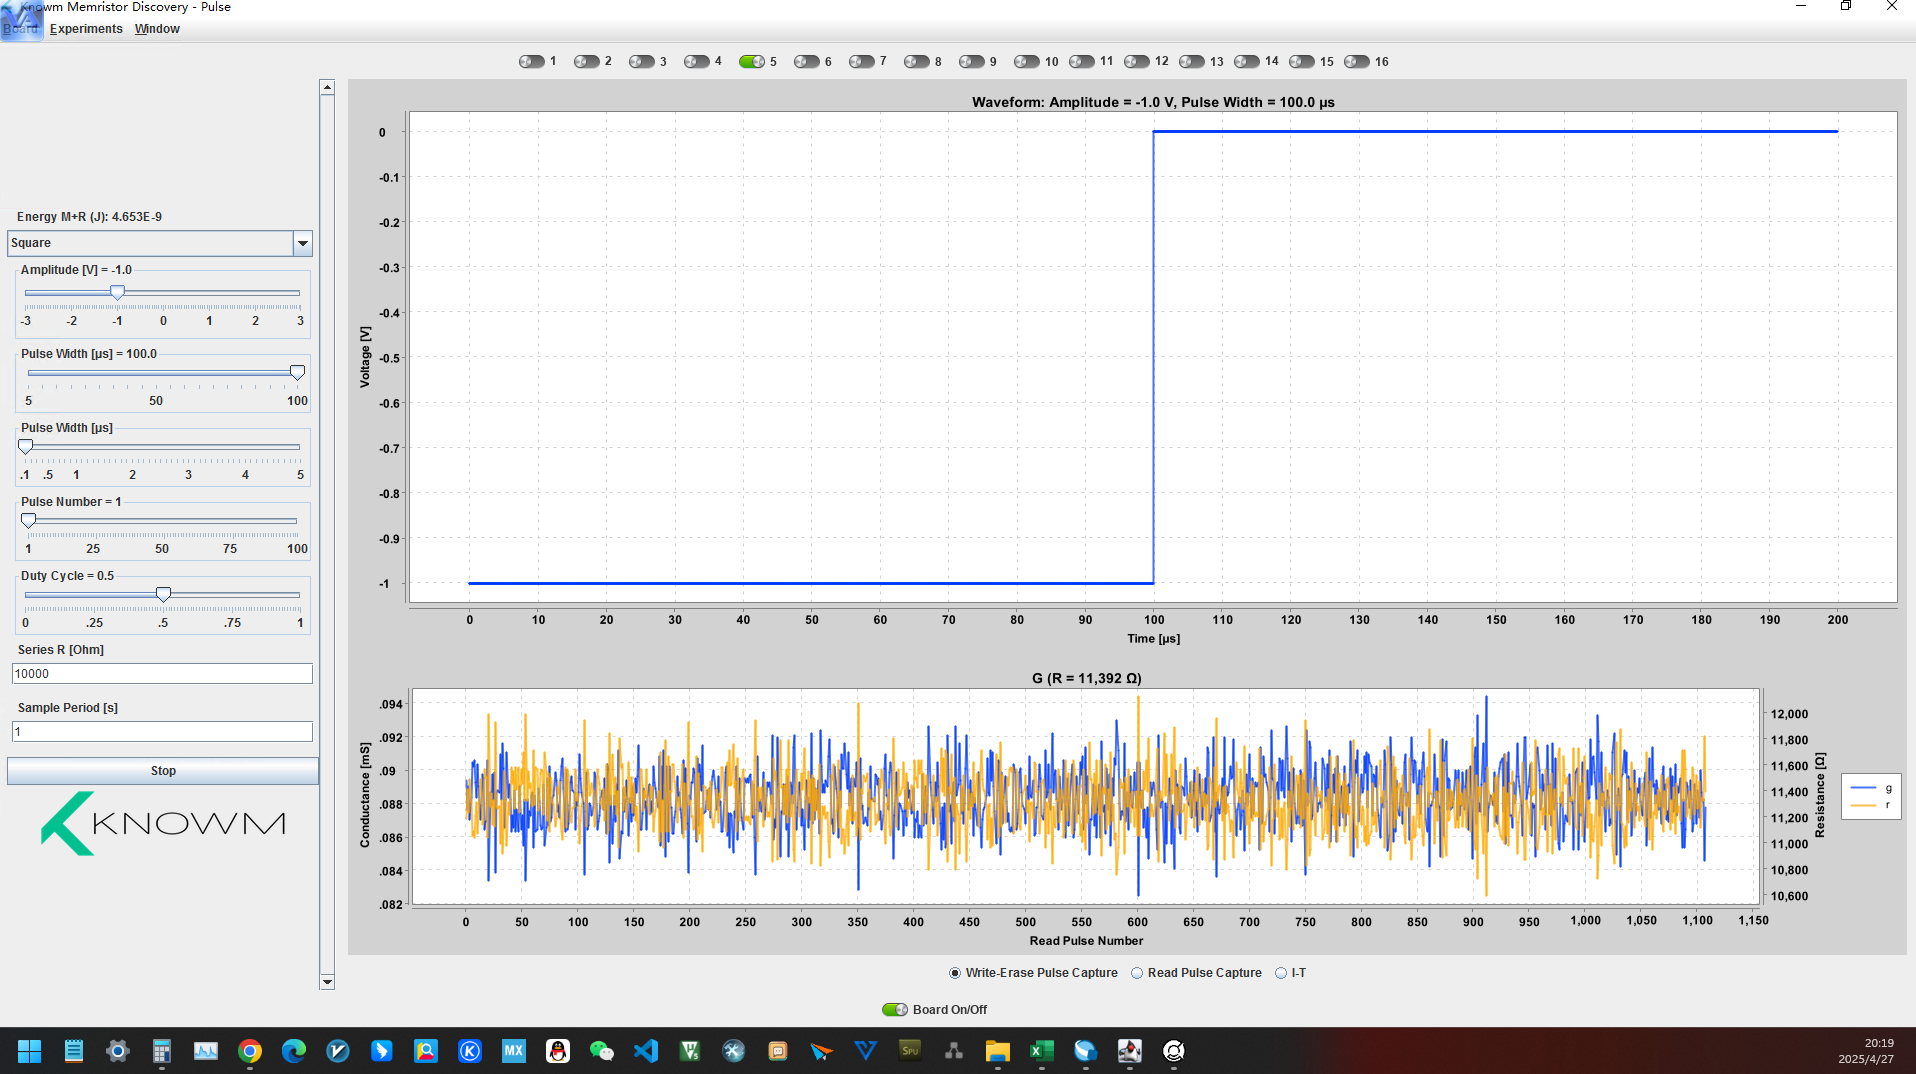
\includegraphics[width=1\textwidth]{figures/U-1T100.png}
        \caption{U=-1,T=100,实验记录}
        \label{fig:U-1T100}
    \end{minipage}
\end{figure}


\end{document}

